\section{Проектирование и разработка программного модуля}
\label{sub:domain:sec_project}
\lstset{style=fsharpstyle}  



\subsection{Определение формул траектории движения}
% cite https://en.wikipedia.org/wiki/Projectile_motion

Движение объекта - это форма движения объекта или частицы (снаряда), которая проецируется вблизи поверхности Земли и движется по искривленной траектории только под действием силы тяжести (в частности, влияние сопротивления воздуха предполагается незначительным). Этот изогнутый путь был показан Галилеем как парабола, но может также быть линией в особом случае, когда он брошен прямо вверх. Изучение таких движений называется баллистикой, а такая траектория является баллистической траекторией. Единственная значимая сила, действующая на объект, - это гравитация, которая действует вниз, тем самым придавая объекту ускорение вниз. Из-за инерции объекта внешняя горизонтальная сила не требуется для поддержания горизонтальной составляющей скорости объекта. Принятие во внимание других сил, таких как трение от аэродинамического сопротивления или внутреннее движение, такое как в ракете, требует дополнительного анализа. Баллистическая ракета - это ракета, управляемая только во время относительно короткой начальной фазы полета, и последующий курс которой регулируется законами классической механики.

Баллистика - это наука о механике, которая касается полета, поведения и воздействия снарядов, особенно пуль, неуправляемых бомб, ракет и т.д., наука или искусство проектирования и ускорения снарядов для достижения желаемой производительности.

Элементарные уравнения баллистики пренебрегают почти каждым фактором, кроме начальной скорости и предполагаемого постоянного ускорения силы тяжести. Практические решения проблемы баллистики часто требуют учета сопротивления воздуха, встречного ветра, движения цели, изменяющегося ускорения под действием силы тяжести, а также в таких задачах, как запуск ракеты из одной точки Земли в другую, вращение Земли. Подробные математические решения практических задач обычно не имеют решений в замкнутой форме и поэтому требуют численных методов решения.

Для начала мы рассмотрим формулы движения объекта учитывая только начальный импульс и гравитационную составляющую. 

Пусть снаряд запускается с начальной скоростью 

\begin{align}\label{math.start_velocity}
	v_0 = v_{0x} i + v_{0y} j.
\end{align}

Компоненты $v_{0x}$ и $v_{0y}$ можно найти если известен начальный угол запуска объекта:

\begin{align}
	& v_{0x} = v_0 \cos \theta, \label{math.start_velocity_x} \\
	& v_{0y} = v_0 \sin \theta. \label{math.start_velocity_y}
\end{align}

\paragraph{Ускорение:}

Поскольку ускорение происходит только в вертикальном направлении, то скорость в горизонтальном направлении постоянна и равна $ v_0 \cos \theta$. Вертикальное движение объекта - это движение объекта во время его свободного падения. Здесь ускорение постоянное и равно $g$. Составляющие ускорения:

\begin{align}
	& a_x = 0 , \label{math.acceleration_x} \\
	& a_y = g . \label{math.acceleration_y}
\end{align}

\paragraph{Скорость:}

Горизонтальная состовляющая скорости остаётся неизменной на протяжении всего полёта. Вертикальная составляющая изменяется линейно, потому что ускорение силы тяжести является постоянным. Ускорения в направлениях $x$ и $y$ могут быть интегрированы для определения компонентов скорости в любое время полёта $t$:

\begin{align}
	& v_x = v_0 \cos \theta , \label{math.velocity_x} \\
	& v_y = v_0 \sin \theta - gt . \label{math.velocity_y}
\end{align}

\paragraph{Перемещение:}

В любой момент времени горизонтальное и вертикальное расположение объекта можно рассчитать по формулам:

\begin{align}
	& x = v_0 t \cos \theta, \label{math.position_x} \\
	& y = v_0 t \sin \theta - \frac12 g t^2. \label{math.position_y}
\end{align}

\paragraph{Коэффициент восстановления:}
%video https://ru.coursera.org/lecture/dynamics1/gipotieza-n-iutona-koeffitsiient-vosstanovlieniia-skorosti-vx0Gj
%cite https://www.top-technologies.ru/ru/article/view?id=33723
%biblio Тригуба А.М., Штагер Е.В. ПРИБЛИЖЕННЫЕ СПОСОБЫ ОЦЕНКИ КОЭФФИЦИЕНТА ВОССТАНОВЛЕНИЯ ПРИ СОУДАРЕНИИ УПРУГИХ ТЕЛ // Современные наукоемкие технологии. – 2014. – № 5-1. – С. 91-93;

%book http://scask.ru/l_book_g_tm.php?id=87
В теории удара физические свойства соударяющихся тел учитываются специальной гипотизой Ньютона, которая представляет собой обработку и обобщение опытных данных. Рассмотрим соударяющиеся тела $A_1$ и $A_2$. Пусть во время удара эти тела соприкасаются друг с другом соответственно в точках $C_1$ и $C_2$. Относительные скорости точки $C_1$ по отношению к телу $A_2$ и $C_2$ по отношению к телу $A_2$ будут равны по величине и противоположны по знаку. Спроектируем какую-нибудь из этих скоростей на нормаль тел $A_1$ и $A_2$ в точке их соприкосновения и обозначим эту проекцию через $v_{n}$. Тогда, согласно гипотезе Ньютона, будем иметь:

\begin{align}
	\left|\frac{v_{n2}}{v_{n1}}\right| = k . \label{math.bounce}
\end{align}

Но при этом уточним, что гипотезу Ньютона об ударе и все выводы, которые из нее получаются, можно применять только в качестве первого приближения к реальным процессам, происходящим в телах при ударе. Это приближение оказывается достаточно хорошим, если при ударе наблюдается только местная деформация тел вблизи точки контакта.



\subsection{Компоненты игровых объектов}

В среде разработки Unity общие правила и характер движения объектов задаются статическим классом \lstinline{Physics2D} (если расчёты проводятся в двумерном пространстве) или классом \lstinline{Physics} (если расчёты проводятся в трёхмерном пространстве).

Одним из самых важных свойств этих классов является свойство \lstinline{gravity}. По умолчанию оно является вектором со значением -9.81 по вертикальной составляющей и 0 по остальным составляющим. Это свойство можно изменять в соответствии с задачами приложения.

\subsubsection{Rigidbody}~

Компонент \lstinline|Rigidbody| (Рисунок \ref{fig:domain:sec_project:rigidbody}) помещает объект под контроль физического движка. Для реалистичного перемещения твёрдых тел, на них воздействуют сила вращения и другие силы. Любой игровой объект должен содержать в себе твёрдое тело, чтобы быть подверженным гравитации, действовать согласно назначенным путём скриптинга силам, или взаимодействовать с другими объектами через физический движок NVIDIA PhysX.
%cite https://docs.unity3d.com/ru/2018.3/Manual/class-Rigidbody.html

\begin{figure}[h]
	\noindent\centering
	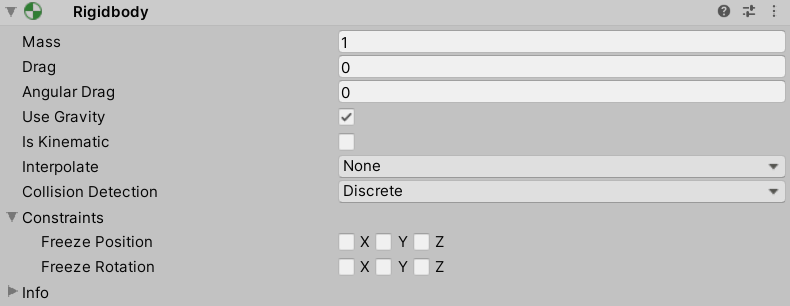
\includegraphics[width=140mm]{rigidbody.png}  
	\caption{Компонент Rigidbody}
	\label{fig:domain:sec_project:rigidbody}
\end{figure}

Настраиваемые свойства \lstinline|Rigidbody|:
\begin{description}
	\item[Mass]	Масса объекта (по умолчанию в килограммах).
	\item[Drag]	Воздушное сопротивление, которое оказывается на объект пока он перемещается под воздействием различных сил. 0 означает отсутствие сопротивления, а бесконечность (infinity) тут же прекращает перемещение объекта.
	\item[Angular Drag]	Воздушное сопротивление, которое оказывается на объект пока он вращается под воздействием силы вращения. 0 означает отсутствие сопротивления. Нельзя остановить вращение объекта путём установки его углового сопротивления (Angular Drag) в бесконечное (infinity) положение.
	\item[Use Gravity]	При включении на объект действует гравитация.
	\item[Is Kinematic]	При включении объект не будет управляться физическим движком, и сможет управляться только при помощи своей трансформации. Полезно при перемещении платформ или если  необходимо анимировать твёрдое тело, которое имеет назначенный HingeJoint.
	\item[Interpolate]	Выбирается одна из опций если была замечена тряска при перемещении твёрдого тела.
	\begin{itemize}
		\item None.	Не применено никакой интерполяции.
		\item Interpolate. Сглаживание транформации основано на трансформации из предыдущего кадра.
		\item Extrapolate. Сглаживание трансформации основано на приблизительной трансформации следующего кадра.
	\end{itemize}
	\item[Collision Detection]	Используется для предотвращения проникновения быстро перемещающихся объектов сквозь другие объекты без определения столкновений.
	\begin{itemize}
		\item Discrete (дискретное). Дискретное обнаружение столкновений со всеми другими коллайдерами в сцене. Другие коллайдеры будут использовать дискретное обнаружение столкновений при тестировании на столкновение с ним. Используется для нормальных столкновений (это значение по умолчанию).
		\item Continuous (непрерывное). Необходимо использовать дискретное обнаружение столкновений с динамическими коллайдерами (с твердым телом) и непрерывное обнаружение столкновений с статическими коллайдерами (без твердого тела). Твердые тела, для которых установлено значение Continuous Dynamic, будут использовать непрерывное обнаружение столкновений при тестировании на столкновение с твердым телом. Другие твердые тела будут использовать дискретное обнаружение столкновений.
		\item Continuous Dynamic (непрерывное динамическое). Используйте непрерывное обнаружение столкновений для объектов GameOject, для которых установлено непрерывное и непрерывное динамическое столкновение. Оно также будет использовать непрерывное обнаружение столкновений со статическими коллайдерами (без твердого тела). Для всех других коллайдеров используется дискретное обнаружение столкновений. Используется для быстро движущихся объектов.
		\item Continuous Speculative (непрерывное спекулятивное). Спекулятивное непрерывное обнаружение столкновений с твердыми телами и коллайдерами. Это также единственный режим обнаружения столкновений, в котором вы можете устанавливать кинематические тела. Этот режим может быть менее дорогим, чем непрерывное обнаружение столкновений.
	\end{itemize}
	\item[Constraints] Ограничения движения твёрдого тела:
	\begin{itemize}
		\item Freeze Position. Выборочно останавливает перемещение твёрдого тела по осям X, Y и Z.
		\item Freeze Rotation. Выборочно останавливает вращение твёрдого тела по осям X, Y и Z.
	\end{itemize}
\end{description}

\subsubsection{Rigidbody2D}~
%cite https://docs.huihoo.com/unity/5.6/Documentation/Manual/class-Rigidbody2D.html

Компонент \lstinline|Rigidbody2D| (Рисунок \ref{fig:domain:sec_project:rigidbody_2d}) помещает объект под контроль физического движка. Многие концепции, знакомые по стандартному компоненту \lstinline|Rigidbody|, переносятся на \lstinline|Rigidbody2D|. Различия в том, что в 2D объекты могут перемещаться только в плоскости XY и могут вращаться только на оси, перпендикулярной этой плоскости.

\begin{figure}[h]
	\noindent\centering
	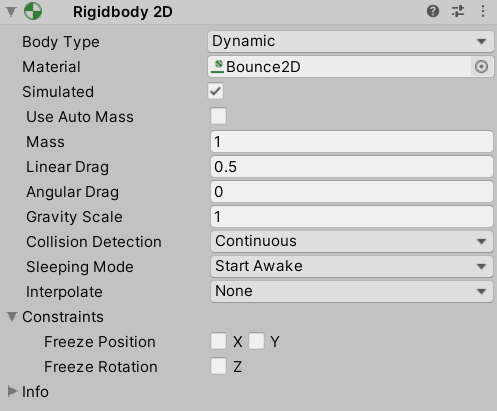
\includegraphics[width=140mm]{rigidbody_2d.png}  
	\caption{Компонент Rigidbody2D}
	\label{fig:domain:sec_project:rigidbody_2d}
\end{figure}

Настраиваемые свойства \lstinline|Rigidbody2D|:
\begin{description}
	\item[Body Type] Есть три варианта для Body Type; каждый определяет фиксированное поведение. Любой Collider2D, прикрепленный к Rigidbody2D, наследует Body Type Rigidbody2D.
	\begin{itemize}
		\item Dynamic. Динамическое твёрдое тело предназначено для движения под симуляцией. Оно обладает полным набором доступных свойств, таких как масса и сопротивление воздуха, и подвержено влиянию силы тяжести. Динамическое тело сталкивается с любым другим типом тела и является наиболее интерактивным из типов телосложения. Это тип тела устанавливается по умолчанию для Rigidbody2D, потому что это наиболее распространенный тип тела для объектов, которые должны двигаться. Это также самый дорогой тип тела из-за его динамичного характера и интерактивности со всем вокруг него. Все свойства Rigidbody2D доступны с этим типом тела.
		\item Kinematic. Кинематическое твёрдое тело разработано для симуляции, но только под явным контролем пользователя. В то время как динамическое твёрдое тело зависит от силы тяжести и силы, кинематическое - нет. По этой причине оно быстрое и требует меньше системных ресурсов, чем динамическое. Кинематическое твёрдое тело разработано для явного перемещения через \lstinline|Rigidbody2D.MovePosition| или \lstinline|Rigidbody2D.MoveRotation|. Необходимо использовать физические методы для обнаружения столкновений и скрипты, чтобы решить, куда и как должно двигаться тело.
		\item Static. Статическое твердое тело разработано так, чтобы вообще не двигаться при симуляции. Если что-то сталкивается с ним, статическое твердое тело ведет себя как неподвижный объект (как будто он имеет бесконечную массу). Это также наименее ресурсоемкий тип тела для использования. Статическое тело сталкивается только с динамическими твёрдыми телами. Столкновение двух статических твёрдых тел не поддерживается, поскольку они не предназначены для перемещения.
	\end{itemize}
	\item[Material] Можно использовать это свойство, чтобы указать общий материал для всех коллайдеров, прикрепленных к конкретному родительскому Rigidbody2D. Collider2D использует свое собственное свойство Material, если оно установлено. Если здесь или в Collider2D не указан материал, по умолчанию используется None (Physics Material 2D). При этом используется материал по умолчанию, который можно установить в окне Physics 2D Settings.
	\item[Simulated] Этот флажок включается, если необходимо, чтобы Rigidbody2D и любые подключенные Collider2D и Joint2D взаимодействовали с физическим моделированием во время выполнения. Если это отключено (флажок снят), эти компоненты не взаимодействуют с симуляцией. Этот флажок установлен по умолчанию.
	\item[Use Auto Mass] Этот флажок устанавливается, если необходимо, чтобы Rigidbody2D автоматически определял массу GameObject из его Collider2D.
	\item[Mass] Определяет массу твердого тела 2D. Заблокировано, если Выбрано «Использовать автоматическую массу».
	\item[Linear Drag] Коэффициент сопротивления, влияющий на позиционное движение.
	\item[Angular Drag] Коэффициент сопротивления, влияющий на вращательное движение.
	\item[Gravity Scale] Коэффициент гравитации. Определяет степень влияния гравитации на GameObject.
	\item[Collision Detection] Определяет, как обнаруживаются столкновения с другими объектами GameObject.
	\item[Sleeping Mode] Спящий режим. Определяет, как GameObject «спит», чтобы сэкономить процессорное время, когда он находится в состоянии покоя.
	\item[Interpolate] Определяет, как движение GameObject интерполируется между обновлениями физики (полезно, когда движение имеет тенденцию к рывкам).
	\item[Constraints] Определяет любые ограничения на движение твёрдого тела.
	\begin{itemize}
		\item Freeze Position. Останавливает перемещение твёрдого тела по осям X и/или Y.
		\item Freeze Rotation. Останавливает вращение твёрдого тела по оси Z.
	\end{itemize}
\end{description}



\subsubsection{Physics Material}~

Физический материал (Рисунок \ref{fig:domain:sec_project:physics_material}) используется для регулировки трения и отскока, возникающего между физическими объектами, когда они сталкиваются.

\begin{figure}[h]
	\noindent\centering
	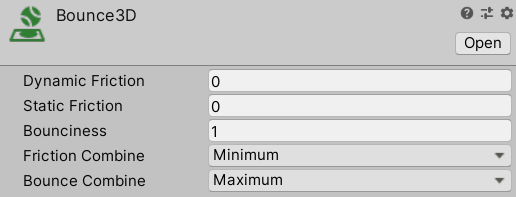
\includegraphics[width=140mm]{physics_material.png}  
	\caption{Компонент Physics Material}
	\label{fig:domain:sec_project:physics_material}
\end{figure}

\begin{description}
	\item[Dynamic Friction]	Трение во время движения. Принимает значения в диапазоне от 0 до 1, где 0 соответствует слабому трению (как на льду), а 1 означает сильное трение, при котором объекту будет сложно двигаться без воздействия внешних сил.
	\item[Static Friction] Трение, использующееся, когда объект лежит на поверхности. Обычно значения бывают в диапазоне от 0 до 1. Значение равное 0 означает отсутствие трения, в то время как значение равное 1 будет означать абсолютное трение (т.е. объектам по такой поверхности будет сложно передвигаться).
	\item[Bounciness] Коэффициент отскока от поверхности (коэффициент восстановления скорости). Значение 0 указывает на отсутствие отскока, а значение 1 указывает на идеальный отскок без потери энергии. Возможны определенные приближения, хотя это может добавить небольшое количество энергии для моделирования.
	\item[Friction Combine]	Как комбинируется между собой трение двух объектов.
	\begin{itemize}
		\item Average. Значения 2 трений усредняются.
		\item Minimum. Из двух значений используется то, что меньше.
		\item Maximum. Из двух значений используется то, что больше.
		\item Multiply. Значения трений умножаются друг на друга.
	\end{itemize}
	\item[Bounce Combine] Как комбинируется упругость двух сталкивающихся объектов. Поддерживает те же режимы, что и Friction Combine.
\end{description}

\subsubsection{Physics Material 2D}~

Физический 2D материал (Рисунок \ref{fig:domain:sec_project:physics_material_2d}) используется для регулировки трения и отскока, возникающего между физическими 2D объектами, когда они сталкиваются.

\begin{figure}[h]
	\noindent\centering
	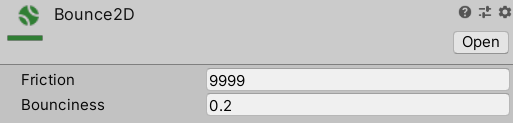
\includegraphics[width=140mm]{physics_material_2d.png}  
	\caption{Компонент Physics Material 2D}
	\label{fig:domain:sec_project:physics_material_2d}
\end{figure}

\begin{description}
	\item[Friction] Коэффициент трения для коллайдера.
	\item[Bounciness] Коэффициент отскока от поверхности (коэффициент восстановления скорости). Значение 0 указывает на отсутствие отскока, а значение 1 указывает на идеальный отскок без потери энергии.
\end{description}


\subsection{Проектирование траектории движения двумерных объектов}

\subsubsection{Линейное движение}~

Для начала спроектируем траекторию линейно движущегося объекта на которое не оказывает влияние сила тяжести и не учитываются пересечения с другими объектами. Для рассчёта положения объекта относительно времени воспользуемся формулами \ref{math.position_x} и \ref{math.position_y} с учётом того, что наша скорость постоянна и не изменяется с течением времени, а так же на объект не воздействует гравитационное ускорение ($g = 0$). У игрового объекта, для которого рассчитываем траектрию движения установим Gravity scale = 0.

Для построения траектории воспользуемся методами, описанными в листинге \ref{listing.trajectory_linear}:

\begin{lstlisting}[style=fsharpstyle, caption={Построение траектории линейно движущегося объекта без воздействия силы тяжести и отскоков}, label=listing.trajectory_linear]
List<Vector3> GetTrajectoryPointsLinear(Vector3 startPosition, Vector3 initialVelocity)
{
	Vector3[] segments = new Vector3[segmentsCount];
		
	segments[0] = startPosition;
		
	Vector3 velocity = initialVelocity;
		
	for (int i = 1; i < segmentsCount; i++)
	{
		float segTime = (velocity.sqrMagnitude != 0) ? segmentLength / velocity.magnitude : 0;
		segments[i] = segments[i - 1] + velocity * segTime;
	}
	
	return segments.ToList();
}
\end{lstlisting}

Запустим приложение и видим, что движение объекта совпадает с построенной траекторией (Рисунок \ref{picture.trajectory_linear}).

\begin{figure}[h]
	\noindent\centering
	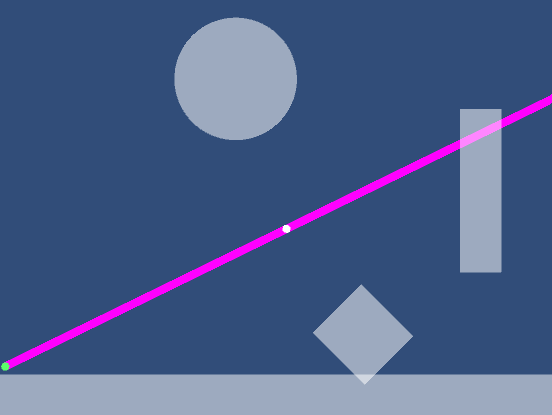
\includegraphics[width=140mm]{trajectory_linear.png}  
	\caption{Движение объекта по линейной траектории без воздействия силы тяжести и отскоков}
	\label{picture.trajectory_linear}
\end{figure}

\subsubsection{Гравитация}~

Добавим условие воздейстия на объект силы гравитации. Для рассчёта положения объекта относительно времени воспользуемся формулами \ref{math.position_x} и \ref{math.position_y} с учётом того, что на объект воздействует гравитационное ускорение ($g = 9.81$). Скорость объекта будет изменяться в соответствии с формулами \ref{math.velocity_x} и \ref{math.velocity_y}. У игрового объекта, для которого рассчитываем траектрию движения установим Gravity scale != 0.

Обновлённый код с учётом воздействия гравитации можно увидеть на листинге \ref{listing.trajectory_with_gravity}:

\begin{lstlisting}[style=fsharpstyle, caption={Построение траектории движущегося объекта c учётом гравитации}, label=listing.trajectory_with_gravity]
List<Vector3> GetTrajectoryPointsWithGravity(Vector3 startPosition, Vector3 initialVelocity)
{
	Vector3[] segments = new Vector3[segmentsCount];
	
	segments[0] = startPosition;
	
	Vector3 velocity = initialVelocity;
	
	var gravityScale = objectPrefab.GetComponent<Rigidbody2D>().gravityScale;
	
	for (int i = 1; i < segmentsCount; i++)
	{
		float segTime = (velocity.sqrMagnitude != 0) ? segmentLength / velocity.magnitude : 0;
		segments[i] = segments[i - 1] + velocity * segTime + Physics.gravity * gravityScale * segTime * segTime / 2;
		velocity += Physics.gravity * gravityScale * segTime;
	}
	
	return segments.ToList();
}
\end{lstlisting}

Запустим приложение и видим, что движение объекта совпадает с построенной траекторией (Рисунок \ref{picture.trajectory_with_gravity}).

\begin{figure}[h]
	\noindent\centering
	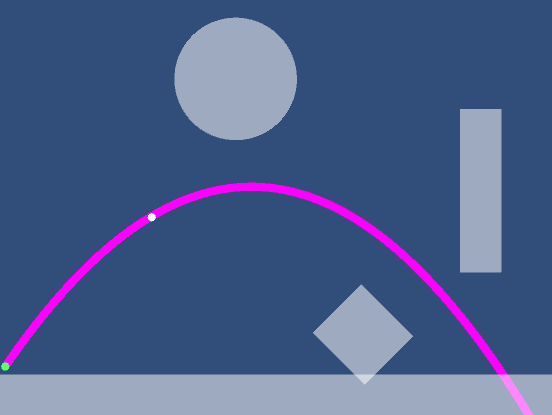
\includegraphics[width=140mm]{trajectory_with_gravity.png}  
	\caption{Движение объекта по траектории под воздействием силы тяжести}
	\label{picture.trajectory_with_gravity}
\end{figure}

\subsubsection{Упругий отскок}~

Для проверки пересечения с другими игровыми объектами мы используем статический метод \lstinline|Physics2D.CircleCast|. Он пускает объект в виде круга из указанной точки в указанном направлении на указанное расстояние. Если на этом расстоянии находится какой-либо другой объект, то возвращается объект \lstinline|RaycastHit2D|, содержащий такие данные о столкновении как точка пересечения, нормаль к точке пересечения, расстояние от начальной точки, \lstinline|Collider2D|, \lstinline|Rigidbody2D| и \lstinline|Transform| объекта, с которым произошло перечечение. Для игрового объекта, для которого рассчитываем траекторию движения установим \lstinline|PhysicsMaterial2D| с Bounciness = 1.

Обновлённый код с учётом воздействия гравитации можно увидеть на листинге \ref{listing.trajectory_reflect}:

\begin{lstlisting}[style=fsharpstyle, caption={Построение траектории движущегося объекта c учётом упругих отскоков от других объектов}, label=listing.trajectory_reflect]
List<Vector3> GetTrajectoryPointsReflect(Vector3 startPosition, Vector3 initialVelocity)
{
	Vector3[] segments = new Vector3[segmentsCount];
	
	segments[0] = startPosition;
	
	Vector3 velocity = initialVelocity;
	
	var gravityScale = objectPrefab.GetComponent<Rigidbody2D>().gravityScale;
	
	for (int i = 1; i < segmentsCount; i++)
	{
		float segTime = (velocity.sqrMagnitude != 0) ? segmentLength / velocity.magnitude : 0;
		
		RaycastHit2D  hit = Physics2D.CircleCast(segments[i - 1], 0.5f, velocity, segmentLength);
		if (hit.collider != null && (Vector2)segments[i - 1] != hit.centroid)
		{
			var hitSegTime = hit.distance / velocity.magnitude;
			segments[i] = segments[i - 1] + velocity * hitSegTime + Physics.gravity * gravityScale * hitSegTime * hitSegTime / 2;
			
			velocity += Physics.gravity * gravityScale * hitSegTime;
			velocity = Vector2.Reflect(velocity, hit.normal);
		}
		else
		{
			segments[i] = segments[i - 1] + velocity * segTime + Physics.gravity * gravityScale * segTime * segTime / 2;
			velocity += Physics.gravity * gravityScale * segTime;
		}
	}
	
	return segments.ToList();
}
\end{lstlisting}

Запустим приложение и видим, что движение объекта совпадает с построенной траекторией (Рисунок \ref{picture.trajectory_reflect}).

\begin{figure}[h]
	\noindent\centering
	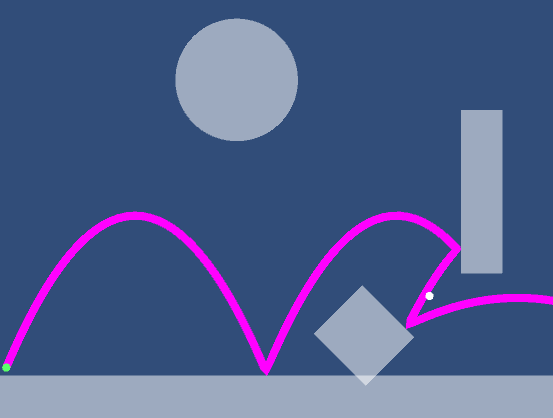
\includegraphics[width=140mm]{trajectory_reflect.png}  
	\caption{Движение объекта c учётом отскоков от других объектов}
	\label{picture.trajectory_reflect}
\end{figure}

\subsubsection{Неупругий отскок}~

Для построения траектории объекта после неупругого столкновения мы воспользуемся формулой \ref{math.bounce}. Учтём, что составляющая скорости объекта коллинеарная нормали изменится в соответствии с коэффициентом восстановления скорости (bounciness) и поменяет направление на противоположное, а касательная составляющая скорости останется неизменной. Для игрового объекта, для которого рассчитываем траектрию движения установим \lstinline|PhysicsMaterial2D| с Bounciness < 1.

Обновлённый код с учётом коэффициента восстановления скорости можно увидеть на листинге \ref{listing.trajectory_bounce}:

\begin{lstlisting}[style=fsharpstyle, caption={Построение траектории движущегося объекта c учётом коэффициента восстановления}, label=listing.trajectory_bounce]
List<Vector3> GetTrajectoryPointsBounce(Vector3 startPosition, Vector3 initialVelocity)
{
	Vector3[] segments = new Vector3[segmentsCount];
	
	segments[0] = startPosition;
	
	Vector3 velocity = initialVelocity;
	
	var bounciness = objectPrefab.sharedMaterial.bounciness;
	var gravityScale = objectPrefab.GetComponent<Rigidbody2D>().gravityScale;
	
	for (int i = 1; i < segmentsCount; i++)
	{
		float segTime = (velocity.sqrMagnitude != 0) ? segmentLength / velocity.magnitude : 0;
		
		RaycastHit2D hit = Physics2D.CircleCast(segments[i - 1], 0.5f, velocity, segmentLength);
		if (hit.collider != null && (Vector2)segments[i - 1] != hit.centroid)
		{
			var hitSegTime = hit.distance / velocity.magnitude;
			segments[i] = segments[i - 1] + velocity * hitSegTime + Physics.gravity * gravityScale * hitSegTime * hitSegTime / 2;
			
			velocity += Physics.gravity * gravityScale * hitSegTime;
			
			var normalVelocity = Vector3.Project(velocity, hit.normal);
			var tangentVelocity = velocity - normalVelocity;
			
			velocity = tangentVelocity - normalVelocity * bounciness;
		}
		else
		{
			segments[i] = segments[i - 1] + velocity * segTime + Physics.gravity * gravityScale * segTime * segTime / 2;
			velocity += Physics.gravity * gravityScale * segTime;
		}
	}
	
	return segments.ToList();
}
\end{lstlisting}

Запустим приложение и видим, что движение объекта совпадает с построенной траекторией (Рисунок \ref{picture.trajectory_bounce}).

\begin{figure}[h]
	\noindent\centering
	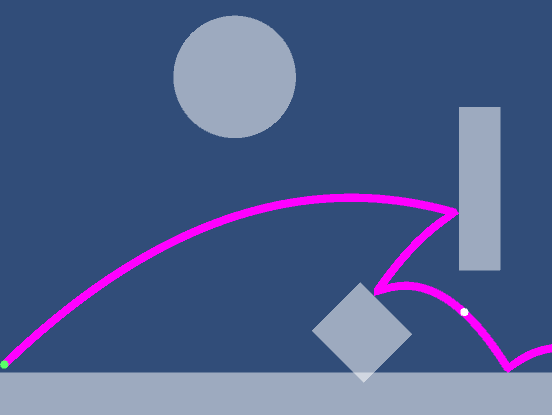
\includegraphics[width=140mm]{trajectory_bounce.png}  
	\caption{Движение объекта c учётом коэффициента восстановления скорости}
	\label{picture.trajectory_bounce}
\end{figure}

\subsubsection{Сопротивление воздуха}~

Сопротивление воздуха воздействующее на тело пока он перемещается для объекта представляется значением \lstinline|Drag|. Можно сказать, что он определяет линейное трение (имеет линейный характер от скорости) и представляет собой значение на которое уменьшается магнитуда скорости в еденицу времени. Метод \lstinline|Mathf.Clamp01(...)| необходим для того чтобы значение скорости в определённый момент не стало отрицательным и объект не двинулся в обратную сторону. Для игрового объекта, для которого рассчитываем траектрию движения установим Drag > 0.

Обновлённый код с учётом сопротивления воздуха можно увидеть на листинге \ref{listing.trajectory_drag}:

\begin{lstlisting}[style=fsharpstyle, caption={Построение траектории движущегося объекта c учётом сопротивления воздуха}, label=listing.trajectory_drag]
List<Vector3> GetTrajectoryPoints(Vector3 startPosition, Vector3 initialVelocity)
{
	Vector3[] segments = new Vector3[segmentsCount];
	
	segments[0] = startPosition;
	
	Vector3 velocity = initialVelocity;
	
	var bounciness = objectPrefab.sharedMaterial.bounciness;
	var drag = objectPrefab.GetComponent<Rigidbody2D>().drag;
	var gravityScale = objectPrefab.GetComponent<Rigidbody2D>().gravityScale;
	
	for (int i = 1; i < segmentsCount; i++)
	{
		float segTime = (velocity.sqrMagnitude != 0) ? segmentLength / velocity.magnitude : 0;
		
		RaycastHit2D hit = Physics2D.CircleCast(segments[i - 1], 0.5f, velocity, segmentLength);
		if (hit.collider != null && (Vector2)segments[i - 1] != hit.centroid)
		{
			var hitSegTime = hit.distance / velocity.magnitude;
			segments[i] = segments[i - 1] + velocity * hitSegTime + Physics.gravity * gravityScale * hitSegTime * hitSegTime / 2;
			
			velocity += Physics.gravity * gravityScale * hitSegTime;
			
			var normalVelocity = Vector3.Project(velocity, hit.normal);
			var tangentVelocity = velocity - normalVelocity;
			
			velocity = tangentVelocity - normalVelocity * bounciness;
			velocity *= Mathf.Clamp01(1f - drag * hitSegTime);
		}
		else
		{
			segments[i] = segments[i - 1] + velocity * segTime + Physics.gravity * gravityScale * segTime * segTime / 2;
			velocity += Physics.gravity * gravityScale * segTime;
			velocity *= Mathf.Clamp01(1f - drag * segTime);
		}
	}
	
	return segments.ToList();
}
\end{lstlisting}

Запустим приложение и видим, что движение объекта совпадает с построенной траекторией (Рисунок \ref{picture.trajectory_drag}).

\begin{figure}[h]
	\noindent\centering
	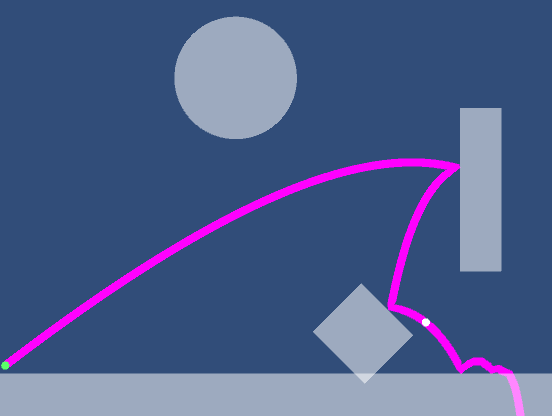
\includegraphics[width=140mm]{trajectory_drag.png}  
	\caption{Движение объекта c учётом сопротивления воздуха}
	\label{picture.trajectory_drag}
\end{figure}

\subsection{Проектирование траектории движения трёхмерных объектов}
В целом построение траектории движения трёхмерного объекта аналогично построению траектории движения двумерного объекта за исключением вычисления вектора скорости после столкновения с другими объектами.

Так для вычисления точки касания и нормали будем использовать метод \lstinline|Physics.SphereCast(...)|. Он пускает объект в виде сферы из указанной точки в указанном направлении на указанное расстояние. Если на этом расстоянии находится какой-либо другой объект, то возвращается объект \lstinline|RaycastHit|, содержащий такие данные о столкновении как точка пересечения, нормаль к точке пересечения, расстояние от начальной точки, \lstinline|Collider|, \lstinline|Rigidbody| и \lstinline|Transform| объекта, с которым произошло перечечение.

Нахождение коэффициента восстановления скорости (отскока) также имеет свои особенности. Когда два тела находятся в контакте, одинаковый эффект отскока применяется к обоим из них в соответствии с выбранным режимом отскока материала (Bounce Combine). Существует особый случай, когда два коллайдера в контакте имеют разные режимы комбинирования. В этом конкретном случае используется функция с наивысшим приоритетом. Порядок приоритетов выглядит следующим образом: Average < Minimum < Multiply < Maximum. Например, если для одного материала установлено значение «Average», а для другого - «Maximum», то используется функция объединения «Maximum», поскольку он имеет более высокий приоритет. Поэтому для рассчёта траектории необходимо учитывать эту особенность материалов.

Код для построения траектории объекта в трёхмерном пространстве можно увидеь на листинге \ref{listing.trajectory_3d}:

\begin{lstlisting}[style=fsharpstyle, caption={Построение траектории трёхмерного движущегося объекта}, label=listing.trajectory_3d]
List<Vector3> GetTrajectoryPoints(Vector3 startPosition, Vector3 initialVelocity)
{
	Vector3[] segments = new Vector3[segmentsCount];
	
	segments[0] = startPosition;
	
	Vector3 velocity = initialVelocity;
	var collider = objectPrefab.GetComponent<Collider>();
	var rigidbody = objectPrefab.GetComponent<Rigidbody>();
	
	var drag = rigidbody.drag;
	var gravityScale = rigidbody.useGravity ? 1 : 0;
	var bounciness = collider.material.bounciness;
	var bounceCombine = collider.material.bounceCombine;
	
	
	for (int i = 1; i < segmentsCount; i++)
	{
		float segTime = (velocity.sqrMagnitude != 0) ? segmentLength / velocity.magnitude : 0;
		
		bool hasHit = Physics.SphereCast(segments[i - 1], 0.5f, velocity, out RaycastHit hit, segmentLength);
		if (hasHit)
		{
			var hitSegTime = hit.distance / velocity.magnitude;
			segments[i] = segments[i - 1] + velocity * hitSegTime + Physics.gravity * gravityScale * hitSegTime * hitSegTime / 2;
			
			velocity += Physics.gravity * gravityScale * hitSegTime;
			
			var normalVelocity = Vector3.Project(velocity, hit.normal);
			var tangentVelocity = velocity - normalVelocity;
			
			var otherBounciness = hit.collider.material.bounciness;
			var otherBounceCombine = hit.collider.material.bounceCombine;
			
			var hitBounceCombine = (PhysicMaterialCombine)Mathf.Max((int)bounceCombine, (int)otherBounceCombine);
			
			var hitBounciness = hitBounceCombine == PhysicMaterialCombine.Average ? (bounciness + otherBounciness) / 2
			: hitBounceCombine == PhysicMaterialCombine.Maximum ? Mathf.Max(bounciness, otherBounciness)
			: hitBounceCombine == PhysicMaterialCombine.Minimum ? Mathf.Min(bounciness, otherBounciness)
			: bounciness * otherBounciness;
			
			velocity = tangentVelocity - normalVelocity * hitBounciness;
			velocity *= Mathf.Clamp01(1f - drag * hitSegTime);
		}
		else
		{
			segments[i] = segments[i - 1] + velocity * segTime + Physics.gravity * gravityScale * segTime * segTime / 2;
			velocity += Physics.gravity * gravityScale * segTime;
			velocity *= Mathf.Clamp01(1f - drag * segTime);
		}
	}
	
	return segments.ToList();
}
\end{lstlisting}

Запустим приложение и видим, что движение объекта совпадает с построенной траекторией (Рисунок \ref{picture.trajectory_3d}).

\begin{figure}[h]
	\noindent\centering
	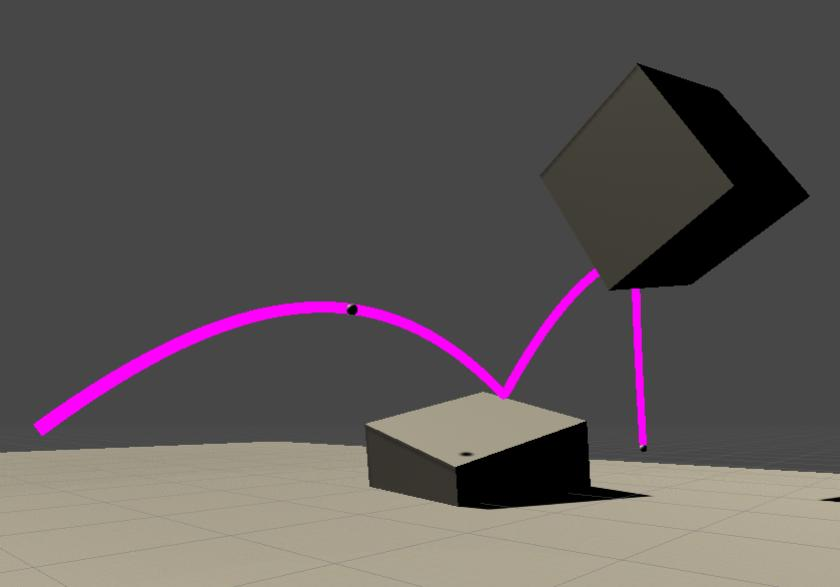
\includegraphics[width=140mm]{trajectory_3d.jpg}  
	\caption{Движение трёхмерного объекта}
	\label{picture.trajectory_3d}
\end{figure}




